\documentclass{article}
\usepackage{packages}
\usepackage{macros}

\title{Size Change Termination Condition for Injective Relations}
\author{Stefano Berardi}
\date{April, 2025}

\begin{document}

\maketitle

\section{Introduction}
\textit{Size change termination}, originally introduced in \cite{Lee1}, is a method used to prove the termination of recursive functions. The main idea behind size change termination lies in Fermat's proof principle of infinite descent: To proof a proposition $P$, assume $P$ is false and reach a contradiction by constructing an infinite descending chain in a well-order. This principle can be applied in the context of recursive functions as follows: if the parameters of a function belong to a well-order, we can assume the function execution does not terminates, and derive a contradiction by forming an infinite descending chain with the values of the parameters. These infinite descending chains are formed by analyzing the relationships between the parameters of the function in each recursive call. Each relationship is captured by a structure known as the \textit{size change graph}, which provides an abstract way to define how the parameters change during program execution. To understand the general idea behind this method, lets consider the following example of the Ackermann function, taken from \cite{Lee2}: 


\begin{figure}[ht]
  \centering
  % Minipage for the code listing
  \begin{minipage}[b]{0.45\textwidth}
    \begin{lstlisting}[basicstyle=\normalsize\ttfamily]
a(m,n) = if m=0 then n+1 else
         if n=0 then *${}^{1}$*a(m-1,1) else
         *${}^{2}$*a(m-1,*${}^{3}$*a(m,n-1))
    \end{lstlisting}
  \end{minipage}
  % Minipage for the first TikZ figure
  \begin{minipage}[b]{0.25\textwidth}
    \centering
    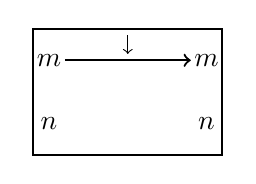
\begin{tikzpicture}[scale=0.8]
      % Draw the rectangle frame
      \draw[thick] (-1.5,-1.0) rectangle (1.5,1.0);
      % Place the nodes
      \node at (-1.25, 0.5) {$m$};
      \node at (1.25, 0.5) {$m$};
      \node at (-1.25, -0.5) {$n$};
      \node at (1.25, -0.5) {$n$};
      % Draw arrows m -> m
      \draw[thick, ->] (-1.0,0.5) -- (1.0,0.5);
      \draw[->] (0, 0.9) -- (0, 0.6);
    \end{tikzpicture}
    
    \vspace{0.1cm}
    
    $G_1, G_2$
  \end{minipage}
  % Minipage for the second TikZ figure
  \begin{minipage}[b]{0.25\textwidth}
    \centering
    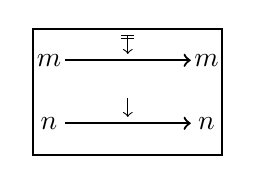
\begin{tikzpicture}[scale=0.8]
      % Draw the rectangle frame
      \draw[thick] (-1.5,-1.0) rectangle (1.5,1.0);
      % Place the nodes
      \node at (-1.25, 0.5) {$m$};
      \node at (1.25, 0.5) {$m$};
      \node at (-1.25, -0.5) {$n$};
      \node at (1.25, -0.5) {$n$};
      % Draw arrows m -> m
      \draw[thick, ->] (-1.0,0.5) -- (1.0,0.5);
      \draw (-0.1, 0.9) -- (0.1, 0.9);
      \draw (-0.1, 0.85) -- (0.1, 0.85);
      \draw[->] (0, 0.9) -- (0, 0.6);
      % Draw arrows n -> n
      \draw[thick, ->] (-1.0,-0.5) -- (1.0,-0.5);
      \draw[->] (0, -0.1) -- (0, -0.4);
    \end{tikzpicture}
    
    \vspace{0.1cm}
    
    $G_3$
  \end{minipage}
  \caption{Definition of the Ackermann function \texttt{a} and size change graphs $G_1$, $G_2$ and $G_3$}
  \label{figFuncF}
\end{figure}

For each recursive call, labeled with 1,2 and 3, we can respectively define the size change graphs $G_1$, $G_2$ and $G_3$, where the edges $x \xrightarrow{\gamma} y$ represent the relationship between the values of the parameters initially passed to the function, and the values after each recursive call. When $\gamma = \ \downarrow$, it specifies that the value of $x$ is strictly less than the value of $y$, and when $\gamma = \downmapsto$ , it specifies that the value of $x$ is less than or equal to the value of $y$. Using these graphs we can then analyze the function's execution: assume a hypothetical infinite execution of the program. This will induce an infinite sequence of recursive calls $c = c_1c_2c_3...$ where every $c_i \in \{1,2,3\}$, which also induces an infinite sequence of size change graphs $G_{c_1}G_{c_2}G_{c_3}...$ It is then possible to compose these graphs, to form infinite paths using the relations between each one of the variables. For example, suppose we get an infinite execution $(13)^{\omega}$, i.e. the recursive call 1 and 3 are used infinitely one after the other. This induces the sequences of graphs $(G_1G_3)^{\omega}$ and the infinite path $m \xrightarrow{\downarrow} m \xrightarrow{\downmapsto} m \xrightarrow{\downarrow} m ...$ over the variable $m$, which progresses infinitely often and implies that this infinite execution is impossible.





\textcolor{red}{\begin{enumerate}
    \item Continue with Cyclic proofs (cite ikebuchi) and use an example to explain the intuition why GTC is STC.
    \item Explain how this can be abstracted in a more general way for any circular system with progressing condition
    \item Explain why in general circular proof systems satisfy injectivity
    \item state what is the objective of the paper
\end{enumerate}}


%BIBLIOGRAPHY:
\bibliographystyle{alpha}
\bibliography{references}






%    \begin{tikzpicture}[scale=0.8]
      % Draw the rectangle frame
%      \draw[thick] (-1.5,-1.0) rectangle (1.5,1.0);
      % Place the nodes
%      \node at (-1.25, 0.5) {$n$};
%      \node at (1.25, 0.5) {$n$};
%      \node at (-1.25, -0.5) {$m$};
%      \node at (1.25, -0.5) {$m$};
      % Draw arrows n -> m
%      \draw[thick, ->] (-1.0,0.5) -- (1.0,-0.5);
%      \draw[->] (-0.5, 0.7) -- (-0.5, 0.4);
      % Draw arrows m -> m
%      \draw[thick, ->] (-1.0,-0.5) -- (1.0,0.5);
%      \draw[->] (-0.5, -0.4) -- (-0.5, -0.7);
%      \draw (-0.6, -0.4) -- (-0.4, -0.4);
%      \draw (-0.6, -0.45) -- (-0.4, -0.45);
%    \end{tikzpicture}


\end{document}
